%% Requires fithesis2 module (can be downloaded from
%% https://github.com/arax/fithesis2
%% Load document class fithesis2
%% {10pt, 11pt, 12pt}
%% {draft, final}
%% {oneside, twoside}
%% {onecolumn, twocolumn}
%% sudo yum install texlive texlive-babel-czech texlive-hyphen-czech 
 
\documentclass[10pt,final,oneside]{fithesis2}
\pdfoptionpdfminorversion 7

%% Basic packages
\usepackage[czech]{babel}
\usepackage{cmap}
\usepackage[T1]{fontenc}
\usepackage{lmodern}
\usepackage[utf8]{inputenc}
\usepackage{graphicx}

%% Additional packages for colors, advanced
%% formatting options, etc.
\usepackage{color}
\usepackage{microtype}
\usepackage{url}
\usepackage{cslatexquotes}
\usepackage{fancyvrb}
\usepackage[small,bf]{caption}
\usepackage[plainpages=false,pdfpagelabels,unicode]{hyperref}
\usepackage[all]{hypcap}
\usepackage{amssymb}
\usepackage{courier}
\usepackage{listings}
\usepackage{pdfpages}

%% Fix long URLs in DVIs
\usepackage{ifpdf}

\ifpdf
\else
  \usepackage{breakurl}
\fi

%% Packages used to generate various lists
\usepackage{makeidx}
\makeindex

\usepackage[acronym]{glossaries}
\makeglossaries

\newacronym{rest}{REST}{REpresentationl State Tranfer}

\newacronym{eu}{EU}{Evropská Unie}

\newacronym{cors}{CORS}{Cross-origin Resource Sharing}

\newacronym{is}{IS}{Informační systém}

\newacronym{muni}{MUNI}{Masarykova Univerzita}

\newacronym{rdp}{RDP}{Remote Desktop Protocol}

\newglossaryentry{service-oriented-design}{
  name=service-oriented design, 
  description={lalalaa}
}

\newglossaryentry{sla}{
  name=Service-Layer Agreement, 
  description={lalala}
}

\newglossaryentry{api}{ 
  name=API, 
  description={Aplikační rozhraní (API z anglického \emph{Application Programming Interface}) označuje rozhraní poskytované k integraci programů třetích stran}
}

\newglossaryentry{resource-based-model} {
  name=resource-based model, 
  description={lalala}
}

\newglossaryentry{json}{
  name=JSON,
  description={Průběžná integrace (CI z anglického \emph{Continuous Integration}) označuje souhrn nástrojů použitých k průběžné kontrole zdrojového kódu. Typicky sem patří spouštění testů, kontrola kvality kódu, statická analýza kódu a podobně}
}

\newglossaryentry{cms}{ 
  name=CMS, 
  description={Systém pro správu obsahu (CMS z anglického \emph{Content Management System}) označuje typicky internetovou aplikaci umožňující uživatelům úpravu obsahu. Bývá také označován jako redakční systém}
}

\newglossaryentry{css}{ 
  name=CSS, 
  description={Kaskádové styly (CSS z anglického \emph{Cascading Style Sheets}) je jazyk určený k popisu vzhledu webových stránek}
}

\newglossaryentry{cvs}{
  name=CVS,
  description={Systém ke správě verzí projektu (CVS z anglického \emph{Concurrent Version System}) slouží k ukládání historie verzí zdrojového kódu}
}

\newglossaryentry{deployment}{
  name=nasazení,
  description={Proces instalace projektu na typicky vzdálený server a spuštění případných migračních skriptů a pododbně}
}

\newglossaryentry{framework}{
  name=framework,
  description={Označení pro nástroj ulehčující vývoj software, typicky obsahující podpůrné knihovny, nástroje či popisující správný postup vývoje}
}

\newglossaryentry{mediaqueries}{
  name=@Media-Queries,
  description={Pravidla jazyka CSS umožňující podmínit použití vnořených pravidel dle určíté podmínky (typicky rozlišení monitoru a podobně)}
}

\newglossaryentry{opensource}{
  name=open-source,
  description={Software jehož zdrojový kód je volně dostupný a dle licence i upravitelný}
}

\newglossaryentry{responsive}{
  name=responsivní web design, 
  description={Způsob stylování webových dokumentů, při kterém je brán ohled na různá rozlišení klientských zařízení (telefon, tablet, počítač)}
}

\newglossaryentry{servlet}{
  name=Servlet,
  description={Program v jazyce JAVA, který na straně serveru zpracovává HTTP požadavky}
}

\newglossaryentry{ssh}{
  name=SSH,
  description={Zabezpečený komunikační protokol (z anglického \emph{Secure Shell} používaný v TCP/IP sítích}
}

\newglossaryentry{wysiwyg}{
  name=WYSIWYG, 
  description={Zkratka anglického \emph{,,What you see is what you get''}, doslowně přeloženo jako ,,dostaneš to co vidíš''. Používá se pro označení editorů html kódu, které poskytují formátování pomocí tlačítek a výstup automaticky konvertují do html kódu}
}

\newglossaryentry{url}{
  name=URL,
  description={Jednotný lokátor zdrojů (URL z anglického \emph{Uniform Resource Locator} označuje řetězec znaků definující jedinečné umístění}
}

\newglossaryentry{ruby} {
  name=Ruby, 
  description={}
}

\newglossaryentry{session} {
  name=relace,
  description={Také jako sezení, označuje přetrvávající spojení mezi serverem a klientem}
}

\newglossaryentry{uco} {
  name=UČO, 
  description={Unikátní číslo studenta či zaměstnance vysoké školy}
}

\newglossaryentry{xss} {
  name=XSS, 
  description={Využití bezpečnostních chyb stránky (XSS z anglického \emph{Cross-Site Scripting} za pomoci narušení skriptů stránek a podstrčení změněného kódu či dat}
}


%% Use STAR and CIRCLE signs for nested
%% itemized lists
\renewcommand{\labelitemii}{$\star$}
\renewcommand{\labelitemiii}{$\circ$}

%% Title page information
\thesistitle{Service-oriented architecture versioning analysis and application in corporate environment}
\thesissubtitle{Diploma thesis}
\thesisstudent{Ivana Haraslínová}
\thesiswoman{false} %% Important when using Slovak or Czech lang
\thesisfaculty{fi}  %% {fi, eco, law, sci, fsps, phil, ped, med, fss}
\thesislang{en}     %% {en, sk, cs}
\thesisyear{2014}
\thesisadvisor{Ing. Leonard Walletzký, Ph.D}

%% Beginning of the document
\begin{document}

%% Front page with a logo and basic thesis information
\FrontMatter
\ThesisTitlePage


%% Thesis declaration (required)
\begin{ThesisDeclaration}
  \DeclarationText
  \AdvisorName
\end{ThesisDeclaration}

%%\chapter*{Zadání práce}
%%

\begin{ThesisThanks}

\end{ThesisThanks}

\begin{ThesisAbstract}

\end{ThesisAbstract}

%% Keywords (required)git
\begin{ThesisKeyWords}

\end{ThesisKeyWords}

%% Beginning of the thesis itself
\MainMatter

%% TOC (required)
\tableofcontents

%% Thesis text structured using
%% chapters, sections, subsections, etc.
%%\chapter{Introduction}
\label{chap:introduction}

Service-oriented architecture is popular architectural approach to application development. The requirements on the market are dynamically changing. Applications with service-orientation has properties which better response to the needs of market. They are flexible and have a big amount of modern technologies to be applied to their development. Service-oriented applications consist of layers where one of them contains services. They provide functionality to consumer. The consumer is in layer above and is using the services similarly as any customer which is asking for a service in real world.

Companies oriented this way offer their application as a product. Product can be consumed by more than one customer. Corresponding to the needs of each of the clients implies modifications of application to suit all of requirements. Customers can ask for changes on used application and service provider have to correspond to their requirements. Large-scale changes can have impact on all other customers so the can't be reflected immediately on application. Here origins the challenge of versioning. Versioning strategies and approaches are wide topic. There are many of them, many ideas and applications which are already in use by companies. Some services are versioned having good strategy and some of them are less good. But it can be sait that there is no universal solution how versioning should be done. 

\section{Summary}

This thesis is concerned with the services as one of the layers of service-oriented application. Specially it focuses on versioning of the services and analysis of versioning implementation in corporate environment. 

Second chapter contains a short introduction to service-oriented computing. It is a hierarchically highest concept involving service-oriented architecture, design and other principles. The service-oriented architecture (SOA) is described in more detail. There are its specifications and advantages. Further in chapter there is a section about services as a main element of SOA. There are descriptions of what they are and how are created.

Third chapter deals with the Representational State Transfer (REST). An architectural styles according which services can be designed. REST has its constraints and services has to be designed properly to be RESTful. In the chapter there is a description how to meet REST requirements. REST is composed by a set of elements are enumerated and defined. And finally there is an example of REST service.

Next chapter talks about the versioning of services - what causes a need to create a new version and how the services are versioned. There is a description of versioning strategy. The strategical decisions are done before the services are developed. During the versioning the strategy is applied. There are many approaches to version, two of them are analyzed in detail.

Chapter five is about the versioning access. Provider can make the services available by various approaches. The concrete techniques are listed with their examples and applications on REST services. There is a summary of advantages and disadvantages based on the opinion of experienced programmers. At the end of chapter is a table with example of version access of well-known REST services.

Sixth chapter analyzes and apply the versioning on a real company. It introduces a company's architecture and talk about the versioning strategy. It design a possible evolution and changes within their services.

%What are the services will be described in first part. There is ,. The service oriented architecture (SOA) is described in more detail. %Services are components of the SOA. 


\chapter{Service-oriented computing}
\label{chap:service-oriented computing}
\emph{Service-oriented computing} represents a distributed computing platform. [1] It has its own paradigm, logic, architecture and patterns. It is built on the distributed computing platforms and extends it by new considerations about governance, design layers and technologies suitable for its implementation.
\emph{Service orientation} is a design paradigm, it divides the system into logic units which are separately shaped and can be utilized according to strategic goals and benefits of a requested result.

\section{Service-oriented architecture}
\emph{Service-oriented architecture (SOA)} is a set of best practices for an organization leading to agile architectural model of the system to meet business needs. Result of applied practices is an architecture which corresponds to dynamic market changes. The SOA best practices are describing the human behaviour, there is no list of constraints which have to be followed to obtain a service-oriented architecture. The best practices are designed to resolve specific situations which the organization can meet and depending on them could be selected just a subset of appropriate practices which are necessary to apply.

One of the main advantages of a service-oriented architectural style is its ability to efficiently deal with changes. SOA is based on a decomposition of enterprise IT assets and separation of "stable" IT artifacts (services) from "changeable" artifacts (business processes), orchestrating services into IT solutions (processes) \cite{website:versioning-in-soa}. %(http://msdn.microsoft.com/en-us/library/bb491124.aspx)
The speed of changes in the bussines department is too fast to be passed directly into development and maintance of the monolitic systems. Funcionality of this systems is designed on measure of customer and can't deal easily with changes, often it is needed to interfere in design of whole architecture. SOA offers better support when the business requirements change, the changes are refleted into modification of an existing business process, or if it's needed a new process is created using existing services \ref{sec:services}. There are more approaches how to deal with the changes and one of them is versioning \ref{chap:versioning}.


\section{Services}
\label{sec:services}
Services are the logic units form which is composed the \gls{service-oriented-design}. Every service is standalone object or component. Every service has its own functional context and related capabilities. Each service is deployerd independetly on another one and on the system which use it. It allows the parallel development, one service can be the part of many products of the corporation.
The essence of Service in the SOA context is the business abstraction - that is a representation of funcionality and/or data presented in business context.[Agile architecture].

\subsection{Levels of service} 

There are three levels of how we can interpret the expression \emph{'Service'} in SOA context \cite{agile-architecture}:
\begin{enumerate}
  \item \textbf{Service implementation} \hfill \\
Service implementation is the code performing the logic.
  \item \textbf{Service interface} \hfill \\ 
This level is an entry point to the sevice implmentation, it provides underlying logic to consumers but encapsulating it in a way that consumers can see the implementation. 
  \item \textbf{Abstracted service} \hfill \\
Abstracted service or business service represents a business capability or data. This services can be composed to describe a business process. This is a core abstraction of SOA.
\end{enumerate}

There is a many-to-many relationship between these three entities. Business service can represents muliple interfaces and in the same time one interface can be supported by multiple implementation.

/TODO image

\subsection{Service categories and types} %(http://msdn.microsoft.com/en-us/library/bb491121.aspx)

There are two main types of services. The first type is composed by infrastructural services which provide the facilities and aren't a part of application. To the second type belongs services which are the part of the application and provide main logic.

/TODO decribe services

\begin{description}
  \item[Bus services] can be further divided into 
  \begin{enumerate}
    \item Communication services 
    \item Utility services
  \end{enumerate}
  \item[Application services] consist of   
  \begin{enumerate}
    \item Entity services
    \item Capability services
    \item Activity services
    \item Process services
  \end{enumerate}
\end{description}

/TODO image

\section{Services granularity}
During the analytical part of the service design it can be defined the service granularity. The service granularity describes functional scope of the serivce. When the granularity is fine, it means the service contains little logic. On the other hand there are coarse-grained serices which have complex logic but at the expense of flexibility.
Defining the granularity can help to determine the characteristics of the serivce - its performance or size of message. \cite{soa-contract}S

\section{Approaches to implementation}

\subsection{Evolution of approches}
\subsubsection{WSDL RPC SOAP} 
/TODO form agile arcitecture revolution
 
\subsection{REST}
/TODO WADL

Representational State Transfer, REST is an architectural style for building ditributed hypermedia applications.
Thanks to REST disappeared many issues related to web services, but it comes with some new. This thesis deals with REST style and RESTfull services. \ref{chap:rest}

%%\subsubsection*{\textbf{Guacamole} \hfill \emph{http://guac-dev.org/}}
%%\label{subsec:guacamole}
%% \ref{}.
%%    \item \textbf{[název předmětu 1]} \hfill \\
%%    odkaz na stránku předmětu, obsahující pouze název a informace o spolufinancování \gls{eu}
    
%%\begin{table}
%%  \caption{Základní typy entit v Drupalu}
  %%\label{tab:typy-entit}
  %%\begin{tabular}{ | p{3cm} | l | c | c | }
   %% \hline 
    %%Typ entity & Strojový název & Dostupnost polí & Rozšiřitelnost \\ \hline 
    %%Komentář & comment & \checkmark & \checkmark \\ \hline 
    %%Soubor & file &  & \\ \hline 
    %%Slovník & vocabulary &  & \\ \hline 
    %%Uzel & node & \checkmark & \checkmark \\ \hline 
    %%Uživatel & user & \checkmark & \checkmark \\ \hline 
    %%Záznam slovníku & term & \checkmark & \checkmark \\ \hline             
  %%\end{tabular}
%%\end{table}
%% \emph \emph \texttt.


\chapter{Representative State Transfer (REST)}
\label{chap:rest}

\lstset{frame=none,
  language=JAVA,
  aboveskip=3mm,
  belowskip=3mm,
  showstringspaces=false,
  columns=flexible,
  basicstyle={\small\ttfamily},
  numbers=none,
  breaklines=false,
  breakatwhitespace=false,
  tabsize=3
}

\section{REST architecture}
\label{sec:rest-architecture}

REST is "a set of constraints on the overall architectural approach" \cite{agile-architecture}. Roy Thomas Fielding described REST in his doctoral dissertation as an architectural style. The constraints are applied to obtain desired properties of developed architecture. REST is applicable to \gls{hypermedia} applications where multimedia nodes are connected via hyperlinks.

REST architecture is client-server. The server holds implemented logic of services and encapsulates it under the interfaces. The interfaces are entry points for client. Through them data can be obtained and modified. 

\begin{figure}[htp] \centering{
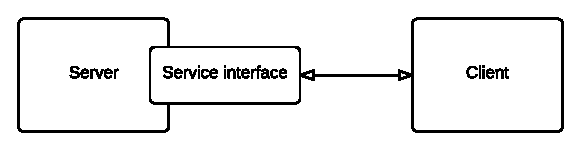
\includegraphics[width=8cm]{img/communication-through-interface.pdf}}
\caption{Client enter the server through the interfaces}
\label{fig:communication-through-interface}
\end{figure} 


The REST is \gls{resource-based-model}. It operates resources named by nouns and actions are provided by HTTP requests. 
REST architecture is a composition of \emph{elements}, \emph{connectors} and \emph{components}. None of them defines specific technology, they are abstractions. The elements abstract a behaviour of components. The components have their roles, the way of interaction among them and interpretation. The REST coposition will be described in Section \ref{sec:rest-composition}

REST has its best practices and constraints. Only services which are built according to this definition can be called \emph{RESTful}. Six constraints characterizing the REST will be described further in Section \ref{sec:constraints}.

\section{Composition of REST}
\label{sec:rest-composition}
As was mentioned above, REST architectional style consist of data elements, connectors and components, shown in Figure \ref{fig:composition-rest}. REST is resource-based, so the main data element is a resource. It is accompanied by resource metadata. Next elemetns are represenatation and its metadata. The last set od data elements are control data. Other than elements REST consists of connectors and components.

\begin{figure}[htp] \centering{
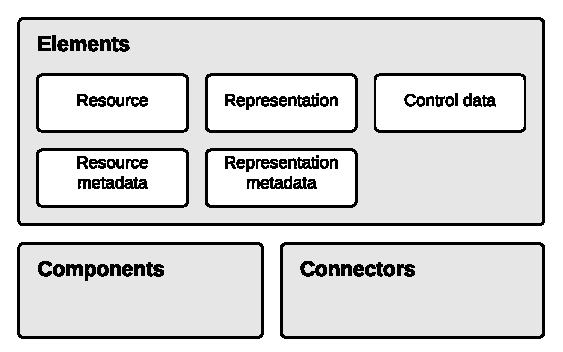
\includegraphics[width=8cm]{img/composition-rest.pdf}}
\caption{Composition of REST}
\label{fig:composition-rest}
\end{figure} 

\subsection{Data elements}
\subsubsection{Resource}
  Resource is an abstraction of information. Any information which can be named by noun can be a resource. "A resource is a conceptual mapping to a set of entities.." \cite{fielding} or set of values. The values can be resource identifiers and representations.
  Resource can be static (for example \emph{an image}) or dynamic (\emph{the time} which dynamically changes).
  
  Examples:
  \begin{center} 
  \begin{lstlisting}
      customer, 
      account, 
      order, 
      ..
  \end{lstlisting} 
  \end{center}

\subsubsection{Resource identifier}
  Serves to identify resources. The resource identifier is assigning a name thanks to which it is possible to reference appropriate resource. The identifier is \gls{url}. It marks a path to reach the resource. A request from client is routed to the specific service and method.
It should be possible to perform the \gls{CRUD} operations with the resources, every operation can be mapped on HTTP method. Having the method and the path the specific operation is performed.

Examples: \\
\begin{center}
\begin{tabular}{l l l}
Method & URL Path & Operation performed \\ \hline
GET & /customers & Retrieves all customers \\
GET & /customers/5 & Retrieves customer with id 5 \\
POST & /customers & Creates new customer \\
PUT & /customers/13 & Updates customer with id 13 \\
DELETE & /customer/2 & Deletes customer with id 2 \\
\end{tabular}
\end{center}

\subsubsection{Representation}
  Representation is used by REST components to perform changes to the resource. The representation stands for a part of (less commonly the whole) resource state. Format of representation's data is called media type and affects the performance of the \gls{hypermedia}. Media types can be proprietary or standardized, from standardized types. There are for comparison \gls{xml} and \gls{json}. JSON format is less verbose and smaller than XML and in consequence in sake of data transmission it would perform faster than a XML representation format.
  
Example of representation:
\begin{center}
  \begin{tabular}[b]{l l}
    In XML format & \begin{lstlisting}
    <?xml version="1.0" encoding="utf-8">
    <customer> 
      <name>Peter<\name> 
      <surname>Smith<\surname> 
      <dateofbirth>20-4-1975<\dateofbirth> 
    <\customer>
    \end{lstlisting} \\
    
\\
    
    In JSON format & \begin{lstlisting}
    {
        "name": "Peter", 
        "surrname": "Smith", 
        "dateofbirth": "20-4-1975"
    }
    \end{lstlisting}
  \end{tabular}
\end{center}

\subsubsection{Representation metadata}
  Representation metadata describes the data of which the representation consists. For example Content-Type defines the \gls{mime-types} of representation sent between client and server. Last-Modified defines the date of last modification of requested object.

  \begin{center}
  \begin{lstlisting}
    {Content-Type: application/json}
    {Content-Type: application/xml}
    {Last-Modified: Thu, 19 May 2015 21:58:55 GMT}
    
  \end{lstlisting}
  \end{center}
  
\subsubsection{Resource metadata}
  Resource metadata describes resources. The examples are Vary which comunicate with proxies whether use a cashed response or request a new ono. Other example is Allow. It defines the allowed methods for a specified resource.
  
  \begin{center}
  \begin{lstlisting}
    {Vary: *}
    {Allow: GET}
  \end{lstlisting}
  \end{center}
  
\subsubsection{Control data}
  "Control data defines the purpose of a message between components, such as the action being requested or the meaning of a response." \cite{fielding}. It can control the caching and parametrize requests. An example can be If-Modified-Since which allows to return a specified response message (304 Not Modified)
  
  \begin{center}
  \begin{lstlisting}
    {If-Modified-Since: Thu, 16 Jun 2014 20:31:00 GMT}
  \end{lstlisting}
  \end{center}
  
  

To summarize the REST elements, every resource has its representation which describes how are resources manipulated in RESTful \gls{api} architecture. The representation is a part or whole resource state. It is transferred between the client and server and has generaly JSON or XML format, but could be in many other formats as well. Representations and resources have their metadata which describe them. Control data affects the messages between client and server.

Client sends a message to server when he wants to operate with a resource. This message is a request. It contains a resource identifier which locates the resource. The request has headers filled by metadata describing the resource and representation. And the body of request involves a representation. An example of a request to create a new customer.

Request:
\begin{center}
  \begin{lstlisting}
     POST /cutomer HTTP/1.1
     Content-Type: application/json
     If-Modified-Since: Thu, 16 Jun 2014 20:31:00 GMT

     {
        "name": "Peter", 
        "surrname": "Smith", 
        "dateofbirth": "20-4-1975"
     }
  \end{lstlisting}
  \end{center}
  
Response:
  \begin{center}
  \begin{lstlisting}
     HTTP/1.1 200 OK 
     Content-Type: application/json
     Allow: POST
     
     {
        "id": 23, 
     }
  \end{lstlisting}
  \end{center}
  
     
The client want to save a representation of customer to the resources. Resources are accessed by URL. Headers are consisting of representation content type which is JSON and control data of modification since specified date. The response message contains headers with content type of a representation and method which is allowed by resource metadata. The response returned an id of created customer. 





\subsection{Connectors}
The connectors encapsulate transfer of representations and access of resources. Connectors are: client, server, cache, resolver, tunnel. %TODO explanation, maybe image

\subsection{Components}
REST components are an abstraction of application unit. The components are origin server, gateway, proxy, user agent. %TODO explanation, maybe image

\section{REST constraints}
\label{sec:constraints}

The REST architectural style has to be developed with respect to its constraints. They are applied to an architecture to create RESTful services. This rules leads to desirable properties of the system, such as performance, scalability, simplicity, modifiability, visibility, portability and reliability. Constraints described below were defined by Roy Thomas Fielding and there are six of them in total.
%%(citacia http://www.restapitutorial.com/lessons/whatisrest.html#)
 
%TODO write about HATEOAS

\subsection{Uniform Interface}
  
Interface stands between client and server. Through the interface client access the server. The REST interface is uniform, client and server always use a fixed set of methods to provide operation over the resources. REST uses \emph{\gls{http} specification}, mostly GET, POST, PUT and DELETE verbs. Despite REST can work with other protocols and define different verbs it uses HTTP operations for practical purpposes. This concept than separates client and server allowing them to develop each part independently and to reduce the coupling between them. %The interface is uniform, so that is easy to understand for both, the server and the client.

Interface is resource-based. Resources are on the server side and the client sents a request process either create, get, update or delete operation over the resource. The request contains a resource identifier in \gls{uri}. It identifies a path to concrete resource. Depending on the type of the request, represention is sent from the client in request and/or from the server in response. The representation is conceptually separated from the resource. It represents appropriate database record.

Resources are manipulated exclusively through the representations. The representation with any metadata attached keeps enough information to modify the resource on the server.

%Sent message represents a clients request or a servers response and it is self-descriptive. It means there is enough information to know how to process the message and the response explicitly defines the cashability.

The representation is sent in a request using HTTP verbs (GET, POST, PUT, DELETE,..) and the URI. Server sends to the client a HTTP response. For illustration a simplified HTTP request and response format is shown in Figure \ref{fig:http}.

\begin{figure}[htp] \centering{
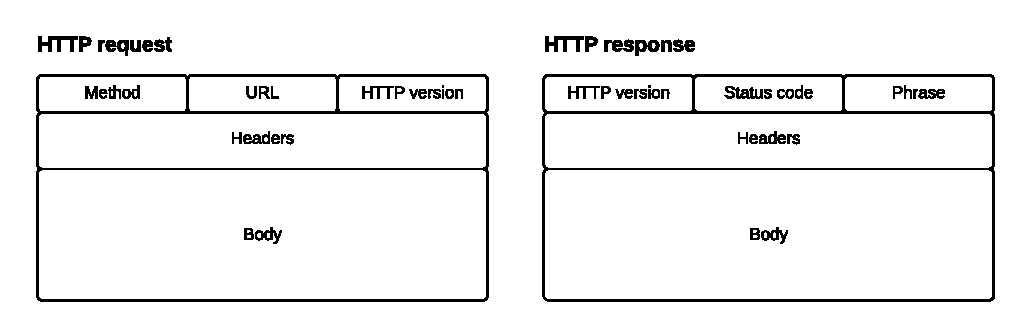
\includegraphics[width=12cm]{img/HTTP.pdf}}
\caption{HTTP request and response}
\label{fig:http}
\end{figure} 

Firts line in the request is called request line. It contains a name of method to be executed over the resource, the URL and HTTP version to be used. Then there are headers and the body for a representation. The response has the fist line starting with HTTP version, than there is a status code with appropriate phrase. Status and phrase reporting whether the request was successful or not.

\subsection{Stateless}
  
Each message is self-descriptive. Request has enough context to be understood and the messages have no state. Any state of a \gls{session} is held just on the client side (for example a logged-in user's session).
The statelessness allows greater scalability, because server doesn't have to communicate with the session, which can be created to carry the state using another architectural style of services. Reliability is improved because of easier recovery of partial failures. Disadvantage is that the sent requests contain repetitive data and the server has lower control over the application's behaviour.

\subsection{Client-server}

RESTful architecture is client-server oriented. There are two separate concerns. It is properly defined what is consumer's side and what are services on server side. Client can’t have direct access to the database, assets or resources. Client-server architecture improves portability of both client and server codes because they are standing alone. The architecture provide simplicity and scalability of server-side code because it doestn't have to include user interface. Client and server are linked together thanks to unified interface and the two can be developed independently.

\subsection{Cacheable}

Server responses (representations) are cacheable. They can be stored to eliminate the interactions with server . Responses can be defined as cashable implicitly, explicitly or negotiated. The cache can be established on server-side, client-side or both as can be seen on Figure \ref{fig:cacheability}. The reason for caching is to reduce interactions over the network. Cached responses are loaded from the cache instead of sending a request to the server. 
Cacheing partially decreses the client-server interaction but improves the scalability and performance. 


\begin{figure}[htp] \centering{
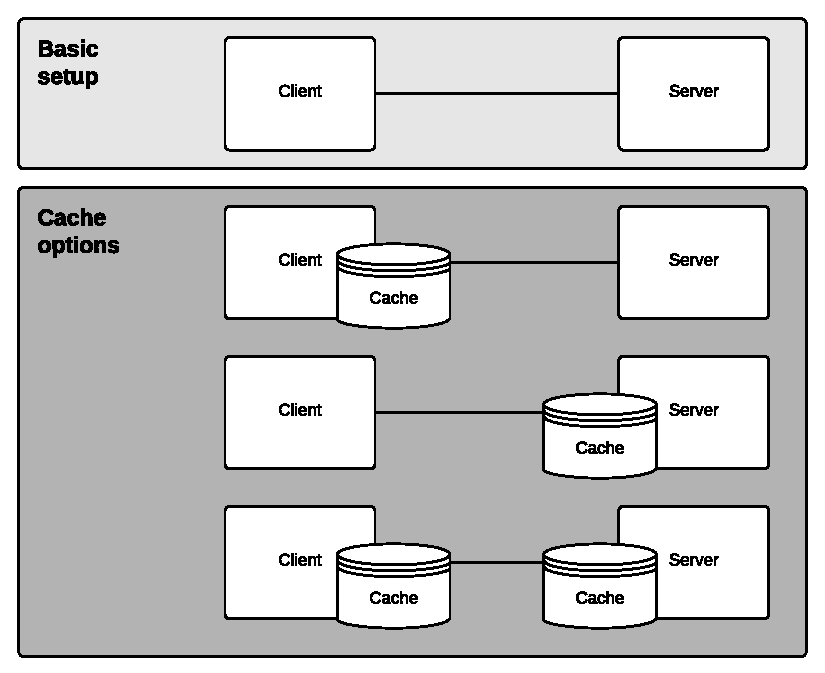
\includegraphics[width=10cm]{img/cacheablity.pdf}}
\caption{Cacheability options}
\label{fig:cacheability}
\end{figure} 

\subsection{Layered system}

This constraint is linked to cashability and client-server principle. System is composed of layers which rapresent independent parts of the system. Example of vertically layered system is shown on Figure \ref{fig:layered-system}. Client is not able to see whether he is communicating directly with the server, or with an intermedia between them. Intermedia improves scalability, provide shared caches and moreover can enforce security policies.

\begin{figure}[htp] \centering{
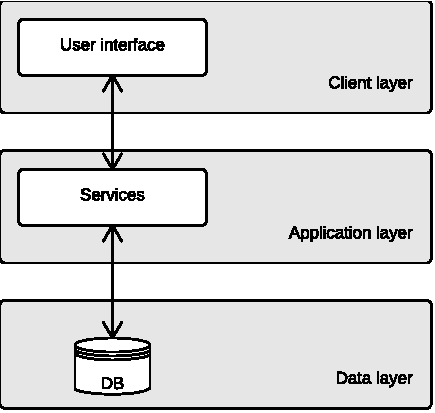
\includegraphics[width=7cm]{img/layered-system.pdf}}
\caption{Layered system example}
\label{fig:layered-system}
\end{figure} 

\subsection{Code on demand}

The logic can be transferred to the client-side. This way the server can temporarily extend or customize the functionality of the client. This can be performed for example by the components like service-side scripts.
This constraint is unique, it is the only one which can be violated and the services can be still RESTful.

\section{Application of REST}

Having the SOA and knowing the constraints of the REST services can be designed. When a company wants to develop a system with RESTful services it has to apply at least the first five of constraints. But it can occur that not all the constraints are profitable for an application. In this case the architecture can forget some of them but the services cannot be further marked as RESTful. This notation doesn't affect services themselves, the result can be still the best design for current application. The RESTful services and their constraints are one of the possible resolutions of architectural style. They are not the universal solution for system architecture.

\subsection{RESTful service example}
There is a corporation with SOA and its services are designed according to REST constraints. One of the services is representing business abstraction of \emph{customers} of the company. Customers can be viewed, created, modified or deleted. The HTTP verbs (GET, POST, PUT, DELETE) are used to perform the operations. 

In designing the service there is considered the notation of \gls{webapi} \gls{framework}. 

Resource identifier is a \gls{uri} address. ASP.NET Web API is composed of \emph{controller} and an \emph{action}. The controller is a class handling the HTTP request and the action is a method of the controller. In this example the controller is \emph{customers}, the action can be \emph{GET} and to identify a specific customer the parameter \emph{name} as to be a part of URI.

\begin{lstlisting}
    GET     customers/getByName/{name} 
\end{lstlisting}

When the client wants to get the customer whose name is \emph{Peter} then the request looks like:

\begin{lstlisting}
    GET     customers/getByName/Peter 
\end{lstlisting}

Thanks to URI the request is routed to specific resource and returns a response. In this response is a representation containing customer identified by requested name. Representation has its media type which are stated in the metadata in this  example it's JSON format:

\begin{lstlisting}
    { 
    "name": "Peter",
    "surname": "Sun",
    "e-mail": "peter.sun@service.com" 
    }
\end{lstlisting}

When the number of customers increases it is not hard to realize that the name identifier is not sufficient. There might be more than just one of the customer named "Peter". The name is obviously not unique and the best solution how to identify an entity is to assign it unique \emph{id} identifier. 

The request and response than look like:
\begin{lstlisting}
    GET     customers/getByName/{id} 
    
    GET     customers/getByName/2 
    
    { 
    "id": 2,
    "name": "Peter",
    "surname": "Sun",
    "e-mail": "peter.sun@service.com" 
    }
\end{lstlisting}


In case the service from the example above is already released and used by client a change can be done. The need of changes like this one is seriously affecting server and client and it is necessary the change is implemented by both of them. How to handle them is a main topic of this thesis and will be explained and analyzed in the rest of this work.

%% \include{tex/vyvoj}
%%\chapter{Conclusion}
\label{chap:conclusion}
To understand the service versioning it is necessary to know the service-oriented architecture (SOA). It was introduced in at the beginning of the thesis. SOA works with services which were described with their relationship to real-world processes. When a company is going to produce an application or system which is service-oriented, it has to analyze the real-world processes and group them by logical units. Those units are services and especially the network operated ones were described in detail.

The thesis outlines Representational State Transfer (REST) architectural style. REST is one of the possible approaches to implementing web services. There are several concepts related to this architecture which need to be followed to obtain RESTful services. 

Versioning is an inevitable part of the service lifecycle. As the real-world changes, the requirements on applications are changing over time as well. The services has to respond to those changes. Every reaction on the change request has to be rooted in versioning strategy. The strategy should be determined during the analytical part. 

Number of approaches to version the services are quite infinite. What is important is a result - provide the service to client. The breaking change require an effort from both to integrate it independently of versioning approach. The main difference between having just one version and more distinct versions accessible at the time has two points of view. From provider side the difference is if he has to wait to client who integrates the service or whether he can deploy new version of API immediately. From client point of view, it can be said, the difference is in amount of accessible versions. 
This thesis analyze two approaches to versioning to demonstrate the differences and impact of each of them on service consumer and provider. This can be helpful to make an overview of approaches for consideration about the versioning strategy for an API. 

Another part of thesis describe consumers access the services version. The URL addresses should be permanent. This results from the REST constraint Uniform interface and connected HATEOAS aspect. After a change of the interface the new version is created. When the services specific versioning approach is used, both API can be deployed and run at the same time. These two versions has a particular way how to access them. The common techniques are enumerated. The techniques can be than further analyzed and customized for particular application. 


This thesis can be further extended several ways. The work presents only analysis of existing versioning techniques. It can be used as a base for creation a versioning strategy of API. Other extension can be deep analysis of Invest s.r.o. API in order to rework the versioning strategy of the company.  




%% Lists of tables and figures, glossary, etc.
\printindex
\printglossary[type=\acronymtype,title={Abbrevations}]
\printglossary
\listoffigures
\listoftables

%% Bibliography from references.bib
\begingroup
\def\tmpchapter{0}
\renewcommand{\chaptername}{}
\renewcommand{\thechapter}{}
%\addtocontents{toc}{\setcounter{tocdepth}{-1}}
\chapter{References}
\renewcommand{\chapter}[2]{}% for other classes

\bibliographystyle{plain}
\bibliography{iharaslinova}

%\addtocontents{toc}{\setcounter{tocdepth}{2}}
\endgroup

%% Additional materials
\appendix

%% End of the whole document
\end{document}
